%!TEX root = ../../thesis.tex


\subsection{Earth's atmosphere, in the NIR}
\todo{move out of intro}
While the Earth's atmosphere is important for an Astronomer's lungs, it can be a nuisance for their ground-based observations.
As light form astronomical sources passes through the atmosphere, its molecular components absorb some of the light, changing spectral components observed by imprinting a transmission spectrum of our atmosphere.
The \ce{H2O} absorption is a key example as it defines the photometric and spectroscopic bands in the \nir{}. \missingfigure{example to point to}.

The correction of observations from the contamination of Earth's atmosphere is a complex process.\textbf{
    The transmission is variable on many different time scales, the water vapour change is rapid, concentrations of atmospheric constituents, to seasonal and longer.}
Such as the increase in atmospheric \ce{CO2} causing anthropamorphic climate change this requires 6\% change to \ce{CO2} line depths since 2000 Molecfit paper?
There is also variation with airmass, which depends on the observation angle in the sky and changes as targets move across the sky during the night.

other constituents, \ce{CO}, \ce{CO2}, \ce{CH4} \ldots{}, angle of observations.

An important consideration in detecting the constituents of planetary atmospheres is the characterization and removal of Earth's telluric lines.

e.g.\ 50\% error in \ce{CO2} detection on Mars atmosphere


Recently~\citet{ulmer-moll_telluric_2018} compared the telluric correction possible from three different synthetic telluric software against the standard star model.
Molecfit, a software from ESO was the most.

This is a growing field and there are other software available too\ldots{}


Water vapour content has rapid variability.
Works such as \citet{snellen_orbital_2010}, fit and remove the telluric variation during a series of observations\footnote{51 spectrum of the same target in 180 minutes for \citet{snellen_orbital_2010}}, to remove telluric lines and detect the absorption lines of exoplanet atmospheres.

\todo{finish this}

\begin{table}
\caption{Standard infrared pass-bands.}

\begin{tabular}{lcc}
    \toprule
    Band &  Central wavelength [\um] & Bandwidth [\um]\\
    \midrule
   Z & 0.9 & 0.06 \\
   Y & 1.05, 0.12 \\
    J & 1.25 & 0.38 \\
    H & 1.65 & 0.48 \\
    K & 2.2 & 0.4 \\
    L & 3.5 & 1.2 \\
    M & 4.8 & 0.6 \\  
    N & 10.6 & 2.5 \\
    Q & 21 & 5.8 \\
    \bottomrule
\end{tabular}
  e.g. \citep{binney_galactic_1998, sterken_astronomical_1992}   
\end{table}



Telluric absorption map
\begin{figure}
    \centering
    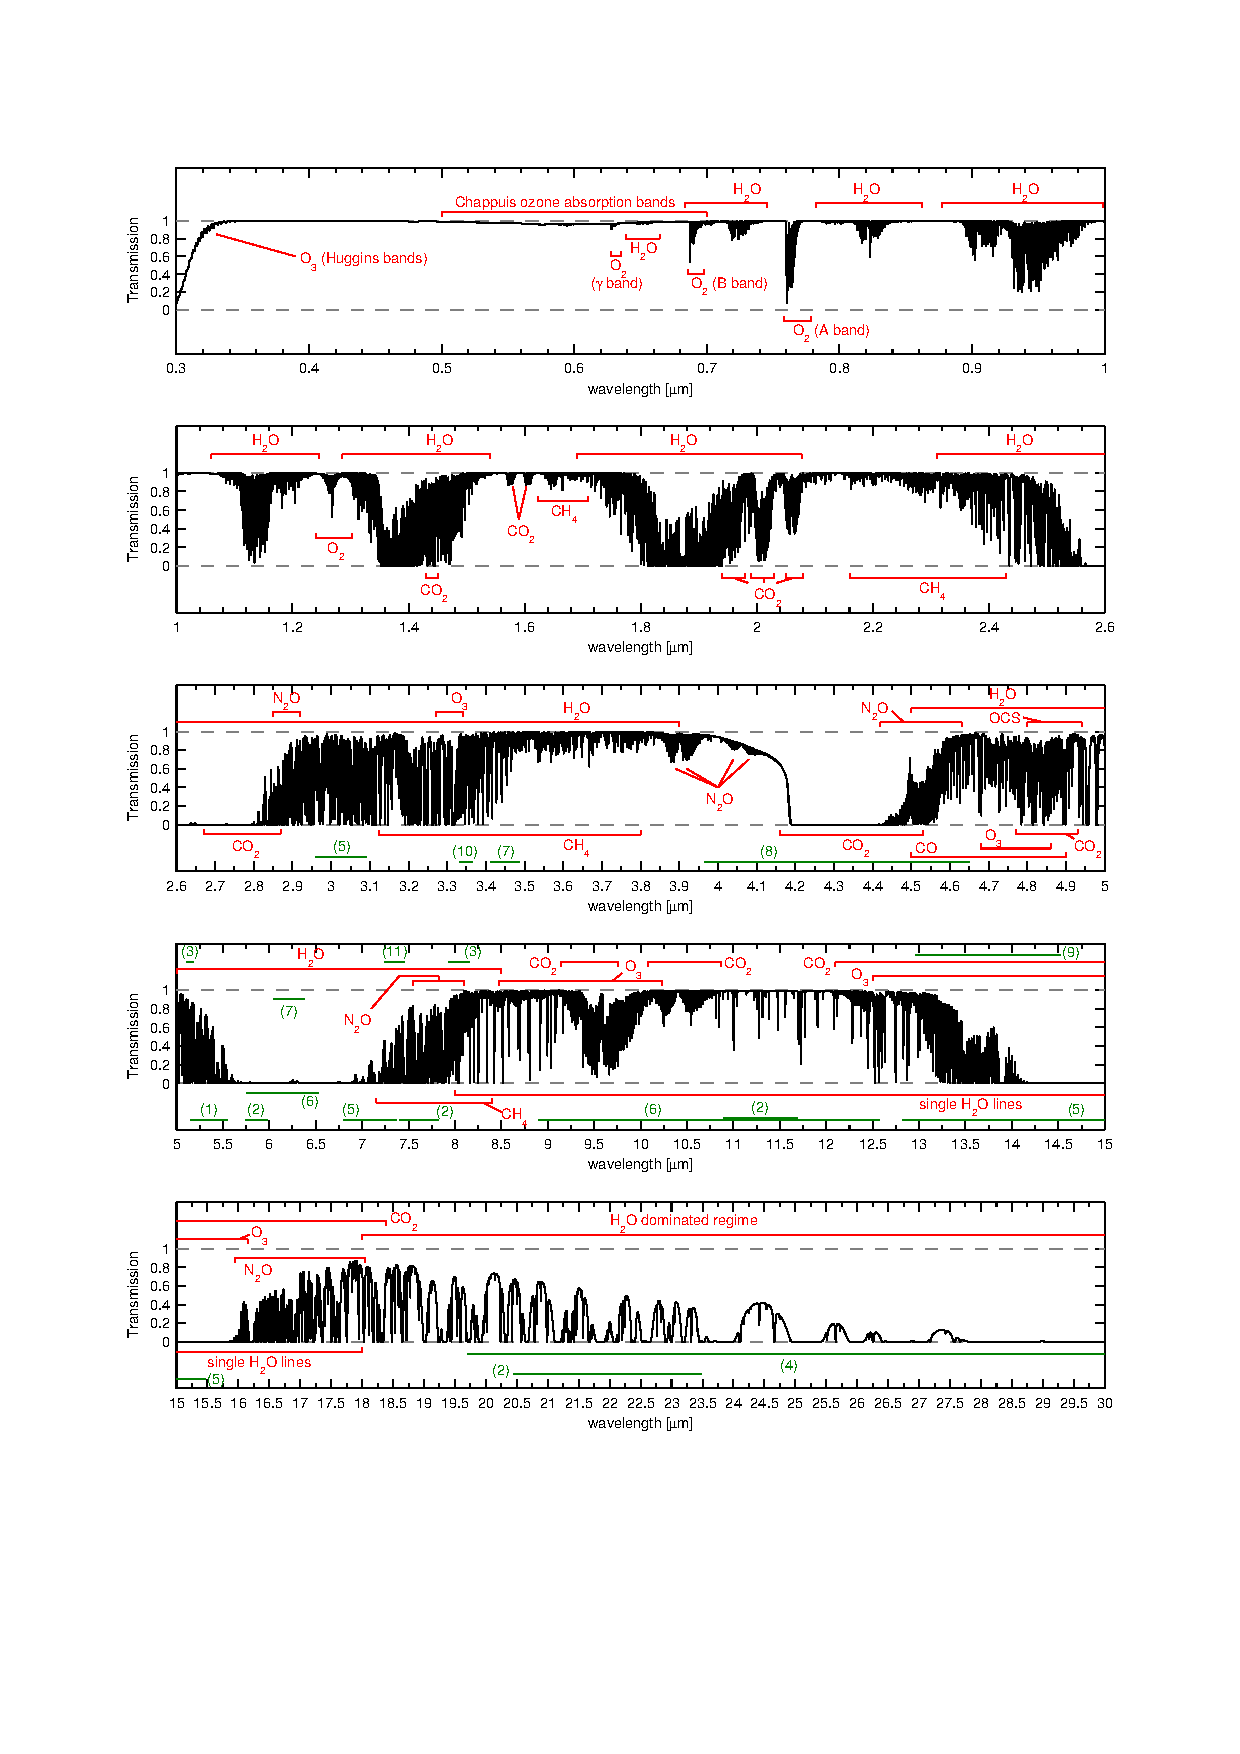
\includegraphics[width=0.9\linewidth]{figures/models/cropped_molecfit_absorbtion}
    \caption{Reproduction of Figure~1 of~\citet{smette_molecfit_2015} showing telluric absorption form 0.30 \um.
        Original caption:\textbf{add more here}}
    \label{fig:croppedmolecfitabsorbtion}
\end{figure}
\todo{Add original caption to~\cref{fig:croppedmolecfitabsorbtion}}